\documentclass[1p]{elsarticle_modified}
%\bibliographystyle{elsarticle-num}

%\usepackage[colorlinks]{hyperref}
%\usepackage{abbrmath_seonhwa} %\Abb, \Ascr, \Acal ,\Abf, \Afrak
\usepackage{amsfonts}
\usepackage{amssymb}
\usepackage{amsmath}
\usepackage{amsthm}
\usepackage{scalefnt}
\usepackage{amsbsy}
\usepackage{kotex}
\usepackage{caption}
\usepackage{subfig}
\usepackage{color}
\usepackage{graphicx}
\usepackage{xcolor} %% white, black, red, green, blue, cyan, magenta, yellow
\usepackage{float}
\usepackage{setspace}
\usepackage{hyperref}

\usepackage{tikz}
\usetikzlibrary{arrows}

\usepackage{multirow}
\usepackage{array} % fixed length table
\usepackage{hhline}

%%%%%%%%%%%%%%%%%%%%%
\makeatletter
\renewcommand*\env@matrix[1][\arraystretch]{%
	\edef\arraystretch{#1}%
	\hskip -\arraycolsep
	\let\@ifnextchar\new@ifnextchar
	\array{*\c@MaxMatrixCols c}}
\makeatother %https://tex.stackexchange.com/questions/14071/how-can-i-increase-the-line-spacing-in-a-matrix
%%%%%%%%%%%%%%%

\usepackage[normalem]{ulem}

\newcommand{\msout}[1]{\ifmmode\text{\sout{\ensuremath{#1}}}\else\sout{#1}\fi}
%SOURCE: \msout is \stkout macro in https://tex.stackexchange.com/questions/20609/strikeout-in-math-mode

\newcommand{\cancel}[1]{
	\ifmmode
	{\color{red}\msout{#1}}
	\else
	{\color{red}\sout{#1}}
	\fi
}

\newcommand{\add}[1]{
	{\color{blue}\uwave{#1}}
}

\newcommand{\replace}[2]{
	\ifmmode
	{\color{red}\msout{#1}}{\color{blue}\uwave{#2}}
	\else
	{\color{red}\sout{#1}}{\color{blue}\uwave{#2}}
	\fi
}

\newcommand{\Sol}{\mathcal{S}} %segment
\newcommand{\D}{D} %diagram
\newcommand{\A}{\mathcal{A}} %arc


%%%%%%%%%%%%%%%%%%%%%%%%%%%%%5 test

\def\sl{\operatorname{\textup{SL}}(2,\Cbb)}
\def\psl{\operatorname{\textup{PSL}}(2,\Cbb)}
\def\quan{\mkern 1mu \triangleright \mkern 1mu}

\theoremstyle{definition}
\newtheorem{thm}{Theorem}[section]
\newtheorem{prop}[thm]{Proposition}
\newtheorem{lem}[thm]{Lemma}
\newtheorem{ques}[thm]{Question}
\newtheorem{cor}[thm]{Corollary}
\newtheorem{defn}[thm]{Definition}
\newtheorem{exam}[thm]{Example}
\newtheorem{rmk}[thm]{Remark}
\newtheorem{alg}[thm]{Algorithm}

\newcommand{\I}{\sqrt{-1}}
\begin{document}

%\begin{frontmatter}
%
%\title{Boundary parabolic representations of knots up to 8 crossings}
%
%%% Group authors per affiliation:
%\author{Yunhi Cho} 
%\address{Department of Mathematics, University of Seoul, Seoul, Korea}
%\ead{yhcho@uos.ac.kr}
%
%
%\author{Seonhwa Kim} %\fnref{s_kim}}
%\address{Center for Geometry and Physics, Institute for Basic Science, Pohang, 37673, Korea}
%\ead{ryeona17@ibs.re.kr}
%
%\author{Hyuk Kim}
%\address{Department of Mathematical Sciences, Seoul National University, Seoul 08826, Korea}
%\ead{hyukkim@snu.ac.kr}
%
%\author{Seokbeom Yoon}
%\address{Department of Mathematical Sciences, Seoul National University, Seoul, 08826,  Korea}
%\ead{sbyoon15@snu.ac.kr}
%
%\begin{abstract}
%We find all boundary parabolic representation of knots up to 8 crossings.
%
%\end{abstract}
%\begin{keyword}
%    \MSC[2010] 57M25 
%\end{keyword}
%
%\end{frontmatter}

%\linenumbers
%\tableofcontents
%
\newcommand\colored[1]{\textcolor{white}{\rule[-0.35ex]{0.8em}{1.4ex}}\kern-0.8em\color{red} #1}%
%\newcommand\colored[1]{\textcolor{white}{ #1}\kern-2.17ex	\textcolor{white}{ #1}\kern-1.81ex	\textcolor{white}{ #1}\kern-2.15ex\color{red}#1	}

{\Large $\underline{12a_{0124}~(K12a_{0124})}$}

\setlength{\tabcolsep}{10pt}
\renewcommand{\arraystretch}{1.6}
\vspace{1cm}\begin{tabular}{m{100pt}>{\centering\arraybackslash}m{274pt}}
\multirow{5}{120pt}{
	\centering
	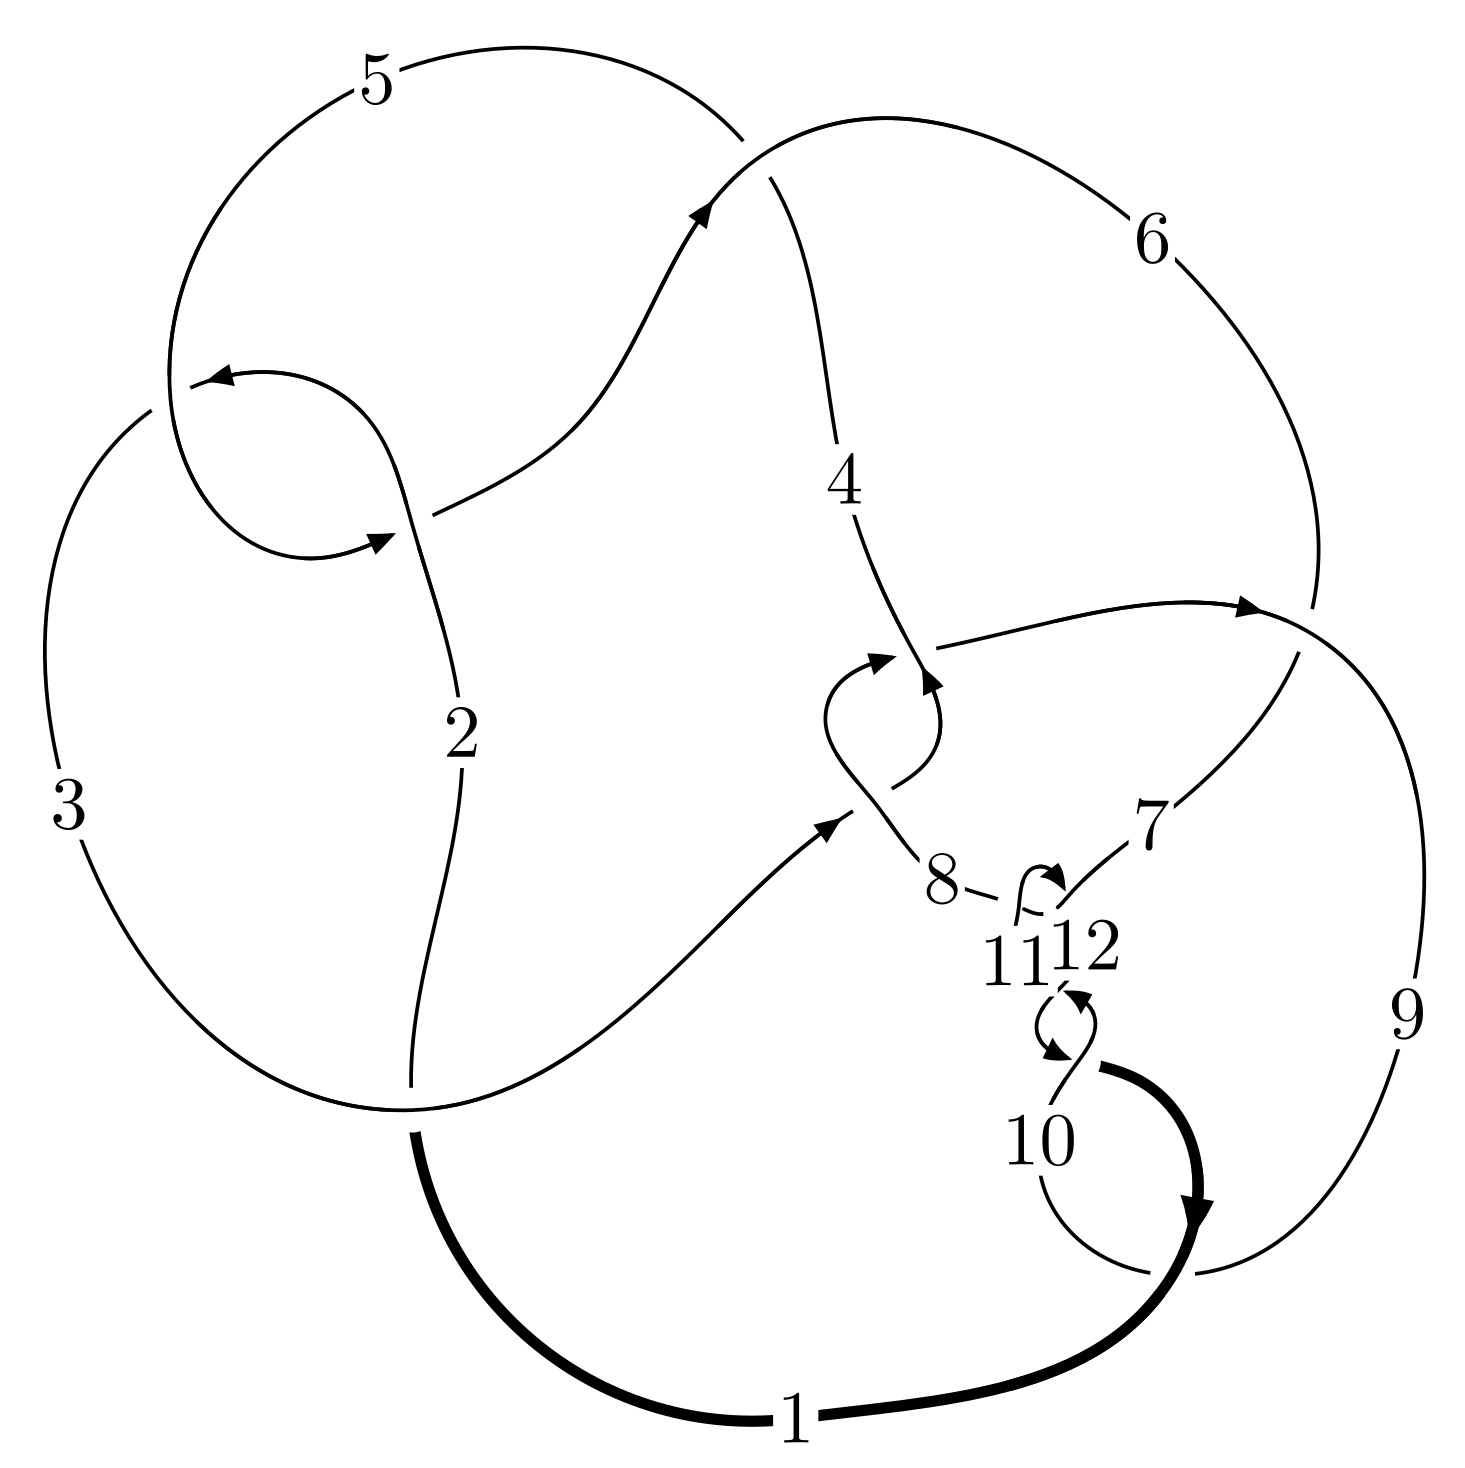
\includegraphics[width=112pt]{../../../GIT/diagram.site/Diagrams/png/925_12a_0124.png}\\
\ \ \ A knot diagram\footnotemark}&
\allowdisplaybreaks
\textbf{Linearized knot diagam} \\
\cline{2-2}
 &
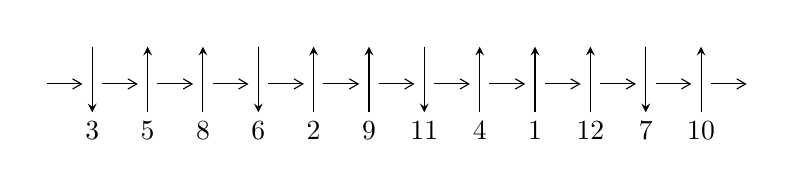
\begin{tikzpicture}[x=20pt, y=17pt]
	% nodes
	\node (C0) at (0, 0) {};
	\node (C1) at (1, 0) {};
	\node (C1U) at (1, +1) {};
	\node (C1D) at (1, -1) {3};

	\node (C2) at (2, 0) {};
	\node (C2U) at (2, +1) {};
	\node (C2D) at (2, -1) {5};

	\node (C3) at (3, 0) {};
	\node (C3U) at (3, +1) {};
	\node (C3D) at (3, -1) {8};

	\node (C4) at (4, 0) {};
	\node (C4U) at (4, +1) {};
	\node (C4D) at (4, -1) {6};

	\node (C5) at (5, 0) {};
	\node (C5U) at (5, +1) {};
	\node (C5D) at (5, -1) {2};

	\node (C6) at (6, 0) {};
	\node (C6U) at (6, +1) {};
	\node (C6D) at (6, -1) {9};

	\node (C7) at (7, 0) {};
	\node (C7U) at (7, +1) {};
	\node (C7D) at (7, -1) {11};

	\node (C8) at (8, 0) {};
	\node (C8U) at (8, +1) {};
	\node (C8D) at (8, -1) {4};

	\node (C9) at (9, 0) {};
	\node (C9U) at (9, +1) {};
	\node (C9D) at (9, -1) {1};

	\node (C10) at (10, 0) {};
	\node (C10U) at (10, +1) {};
	\node (C10D) at (10, -1) {12};

	\node (C11) at (11, 0) {};
	\node (C11U) at (11, +1) {};
	\node (C11D) at (11, -1) {7};

	\node (C12) at (12, 0) {};
	\node (C12U) at (12, +1) {};
	\node (C12D) at (12, -1) {10};
	\node (C13) at (13, 0) {};

	% arrows
	\draw[->,>={angle 60}]
	(C0) edge (C1) (C1) edge (C2) (C2) edge (C3) (C3) edge (C4) (C4) edge (C5) (C5) edge (C6) (C6) edge (C7) (C7) edge (C8) (C8) edge (C9) (C9) edge (C10) (C10) edge (C11) (C11) edge (C12) (C12) edge (C13) ;	\draw[->,>=stealth]
	(C1U) edge (C1D) (C2D) edge (C2U) (C3D) edge (C3U) (C4U) edge (C4D) (C5D) edge (C5U) (C6D) edge (C6U) (C7U) edge (C7D) (C8D) edge (C8U) (C9D) edge (C9U) (C10D) edge (C10U) (C11U) edge (C11D) (C12D) edge (C12U) ;
	\end{tikzpicture} \\
\hhline{~~} \\& 
\textbf{Solving Sequence} \\ \cline{2-2} 
 &
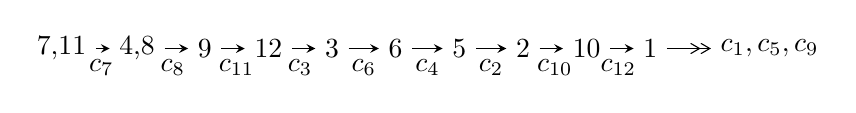
\begin{tikzpicture}[x=23pt, y=7pt]
	% node
	\node (A0) at (-1/8, 0) {7,11};
	\node (A1) at (17/16, 0) {4,8};
	\node (A2) at (17/8, 0) {9};
	\node (A3) at (25/8, 0) {12};
	\node (A4) at (33/8, 0) {3};
	\node (A5) at (41/8, 0) {6};
	\node (A6) at (49/8, 0) {5};
	\node (A7) at (57/8, 0) {2};
	\node (A8) at (65/8, 0) {10};
	\node (A9) at (73/8, 0) {1};
	\node (C1) at (1/2, -1) {$c_{7}$};
	\node (C2) at (13/8, -1) {$c_{8}$};
	\node (C3) at (21/8, -1) {$c_{11}$};
	\node (C4) at (29/8, -1) {$c_{3}$};
	\node (C5) at (37/8, -1) {$c_{6}$};
	\node (C6) at (45/8, -1) {$c_{4}$};
	\node (C7) at (53/8, -1) {$c_{2}$};
	\node (C8) at (61/8, -1) {$c_{10}$};
	\node (C9) at (69/8, -1) {$c_{12}$};
	\node (A10) at (11, 0) {$c_{1},c_{5},c_{9}$};

	% edge
	\draw[->,>=stealth]	
	(A0) edge (A1) (A1) edge (A2) (A2) edge (A3) (A3) edge (A4) (A4) edge (A5) (A5) edge (A6) (A6) edge (A7) (A7) edge (A8) (A8) edge (A9) ;
	\draw[->>,>={angle 60}]	
	(A9) edge (A10);
\end{tikzpicture} \\ 

\end{tabular} \\

\footnotetext{
The image of knot diagram is generated by the software ``\textbf{Draw programme}" developed by Andrew Bartholomew(\url{http://www.layer8.co.uk/maths/draw/index.htm\#Running-draw}), where we modified some parts for our purpose(\url{https://github.com/CATsTAILs/LinksPainter}).
}\phantom \\ \newline 
\centering \textbf{Ideals for irreducible components\footnotemark of $X_{\text{par}}$} 
 
\begin{align*}
I^u_{1}&=\langle 
8 u^{82}-5 u^{81}+\cdots+2 b+6 u,\;-8 u^{82}+24 u^{81}+\cdots+2 a+13,\;u^{83}-3 u^{82}+\cdots+3 u^2+1\rangle \\
I^u_{2}&=\langle 
- u^2 a+b,\;- u^2 a+u^3+a^2- a u+2 u^2- a+2 u,\;u^4+u^3+u^2+1\rangle \\
\\
\end{align*}
\raggedright * 2 irreducible components of $\dim_{\mathbb{C}}=0$, with total 91 representations.\\
\footnotetext{All coefficients of polynomials are rational numbers. But the coefficients are sometimes approximated in decimal forms when there is not enough margin.}
\newpage
\renewcommand{\arraystretch}{1}
\centering \section*{I. $I^u_{1}= \langle 8 u^{82}-5 u^{81}+\cdots+2 b+6 u,\;-8 u^{82}+24 u^{81}+\cdots+2 a+13,\;u^{83}-3 u^{82}+\cdots+3 u^2+1 \rangle$}
\flushleft \textbf{(i) Arc colorings}\\
\begin{tabular}{m{7pt} m{180pt} m{7pt} m{180pt} }
\flushright $a_{7}=$&$\begin{pmatrix}1\\0\end{pmatrix}$ \\
\flushright $a_{11}=$&$\begin{pmatrix}0\\u\end{pmatrix}$ \\
\flushright $a_{4}=$&$\begin{pmatrix}4 u^{82}-12 u^{81}+\cdots-15 u^2-\frac{13}{2}\\-4 u^{82}+\frac{5}{2} u^{81}+\cdots-\frac{13}{2} u^2-3 u\end{pmatrix}$ \\
\flushright $a_{8}=$&$\begin{pmatrix}1\\u^2\end{pmatrix}$ \\
\flushright $a_{9}=$&$\begin{pmatrix}- u^7-2 u^3\\u^7+u^5+2 u^3+u\end{pmatrix}$ \\
\flushright $a_{12}=$&$\begin{pmatrix}- u\\u\end{pmatrix}$ \\
\flushright $a_{3}=$&$\begin{pmatrix}4 u^{82}-12 u^{81}+\cdots- u-\frac{13}{2}\\-4 u^{82}+\frac{7}{2} u^{81}+\cdots-\frac{13}{2} u^2-3 u\end{pmatrix}$ \\
\flushright $a_{6}=$&$\begin{pmatrix}- u^{14}- u^{12}-4 u^{10}-3 u^8-4 u^6-2 u^4+1\\u^{14}+2 u^{12}+5 u^{10}+6 u^8+6 u^6+4 u^4+u^2\end{pmatrix}$ \\
\flushright $a_{5}=$&$\begin{pmatrix}\frac{5}{2} u^{82}-8 u^{81}+\cdots-12 u^2-6\\-\frac{5}{2} u^{82}+u^{81}+\cdots-6 u^2-\frac{5}{2} u\end{pmatrix}$ \\
\flushright $a_{2}=$&$\begin{pmatrix}-\frac{1}{2} u^{79}+u^{78}+\cdots- u^2+\frac{1}{2}\\-\frac{1}{2} u^{81}+u^{80}+\cdots-5 u^4+\frac{1}{2} u^2\end{pmatrix}$ \\
\flushright $a_{10}=$&$\begin{pmatrix}- u^3\\u^3+u\end{pmatrix}$ \\
\flushright $a_{1}=$&$\begin{pmatrix}- u^5- u\\u^5+u^3+u\end{pmatrix}$\\&\end{tabular}
\flushleft \textbf{(ii) Obstruction class $= -1$}\\~\\
\flushleft \textbf{(iii) Cusp Shapes $= \frac{15}{2} u^{82}-8 u^{81}+\cdots+17 u+\frac{25}{2}$}\\~\\
\newpage\renewcommand{\arraystretch}{1}
\flushleft \textbf{(iv) u-Polynomials at the component}\newline \\
\begin{tabular}{m{50pt}|m{274pt}}
Crossings & \hspace{64pt}u-Polynomials at each crossing \\
\hline $$\begin{aligned}c_{1},c_{4}\end{aligned}$$&$\begin{aligned}
&u^{83}+27 u^{82}+\cdots-22 u-1
\end{aligned}$\\
\hline $$\begin{aligned}c_{2},c_{5}\end{aligned}$$&$\begin{aligned}
&u^{83}+5 u^{82}+\cdots-6 u-1
\end{aligned}$\\
\hline $$\begin{aligned}c_{3},c_{8}\end{aligned}$$&$\begin{aligned}
&u^{83}- u^{82}+\cdots+896 u-256
\end{aligned}$\\
\hline $$\begin{aligned}c_{6}\end{aligned}$$&$\begin{aligned}
&u^{83}+3 u^{82}+\cdots-28678 u-6329
\end{aligned}$\\
\hline $$\begin{aligned}c_{7},c_{11}\end{aligned}$$&$\begin{aligned}
&u^{83}+3 u^{82}+\cdots-3 u^2-1
\end{aligned}$\\
\hline $$\begin{aligned}c_{9},c_{10},c_{12}\end{aligned}$$&$\begin{aligned}
&u^{83}-21 u^{82}+\cdots-6 u+1
\end{aligned}$\\
\hline
\end{tabular}\\~\\
\newpage\renewcommand{\arraystretch}{1}
\flushleft \textbf{(v) Riley Polynomials at the component}\newline \\
\begin{tabular}{m{50pt}|m{274pt}}
Crossings & \hspace{64pt}Riley Polynomials at each crossing \\
\hline $$\begin{aligned}c_{1},c_{4}\end{aligned}$$&$\begin{aligned}
&y^{83}+63 y^{82}+\cdots-782 y-1
\end{aligned}$\\
\hline $$\begin{aligned}c_{2},c_{5}\end{aligned}$$&$\begin{aligned}
&y^{83}+27 y^{82}+\cdots-22 y-1
\end{aligned}$\\
\hline $$\begin{aligned}c_{3},c_{8}\end{aligned}$$&$\begin{aligned}
&y^{83}-45 y^{82}+\cdots+770048 y-65536
\end{aligned}$\\
\hline $$\begin{aligned}c_{6}\end{aligned}$$&$\begin{aligned}
&y^{83}-15 y^{82}+\cdots-3774261726 y-40056241
\end{aligned}$\\
\hline $$\begin{aligned}c_{7},c_{11}\end{aligned}$$&$\begin{aligned}
&y^{83}+21 y^{82}+\cdots-6 y-1
\end{aligned}$\\
\hline $$\begin{aligned}c_{9},c_{10},c_{12}\end{aligned}$$&$\begin{aligned}
&y^{83}+85 y^{82}+\cdots+34 y-1
\end{aligned}$\\
\hline
\end{tabular}\\~\\
\newpage\flushleft \textbf{(vi) Complex Volumes and Cusp Shapes}
$$\begin{array}{c|c|c}  
\text{Solutions to }I^u_{1}& \I (\text{vol} + \sqrt{-1}CS) & \text{Cusp shape}\\
 \hline 
\begin{aligned}
u &= -0.343094 + 0.932755 I \\
a &= -2.78793 + 1.29202 I \\
b &= \phantom{-}1.91795 + 0.42351 I\end{aligned}
 & \phantom{-}0.45934 + 5.84256 I & \phantom{-0.000000 } 0 \\ \hline\begin{aligned}
u &= -0.343094 - 0.932755 I \\
a &= -2.78793 - 1.29202 I \\
b &= \phantom{-}1.91795 - 0.42351 I\end{aligned}
 & \phantom{-}0.45934 - 5.84256 I & \phantom{-0.000000 } 0 \\ \hline\begin{aligned}
u &= \phantom{-}0.298458 + 0.943559 I \\
a &= \phantom{-}0.810864 - 1.048410 I \\
b &= -0.268792 + 0.197880 I\end{aligned}
 & \phantom{-}3.34331 - 5.43598 I & \phantom{-0.000000 } 0 \\ \hline\begin{aligned}
u &= \phantom{-}0.298458 - 0.943559 I \\
a &= \phantom{-}0.810864 + 1.048410 I \\
b &= -0.268792 - 0.197880 I\end{aligned}
 & \phantom{-}3.34331 + 5.43598 I & \phantom{-0.000000 } 0 \\ \hline\begin{aligned}
u &= -0.276801 + 0.948551 I \\
a &= \phantom{-}2.78574 - 1.08616 I \\
b &= -1.72816 - 0.44874 I\end{aligned}
 & \phantom{-}4.22365 + 2.71450 I & \phantom{-0.000000 } 0 \\ \hline\begin{aligned}
u &= -0.276801 - 0.948551 I \\
a &= \phantom{-}2.78574 + 1.08616 I \\
b &= -1.72816 + 0.44874 I\end{aligned}
 & \phantom{-}4.22365 - 2.71450 I & \phantom{-0.000000 } 0 \\ \hline\begin{aligned}
u &= -0.151262 + 1.004710 I \\
a &= -2.47403 + 1.00449 I \\
b &= \phantom{-}1.40269 + 0.20603 I\end{aligned}
 & \phantom{-}8.14096 - 5.43626 I & \phantom{-0.000000 } 0 \\ \hline\begin{aligned}
u &= -0.151262 - 1.004710 I \\
a &= -2.47403 - 1.00449 I \\
b &= \phantom{-}1.40269 - 0.20603 I\end{aligned}
 & \phantom{-}8.14096 + 5.43626 I & \phantom{-0.000000 } 0 \\ \hline\begin{aligned}
u &= -0.176749 + 1.004370 I \\
a &= \phantom{-}2.53616 - 1.01779 I \\
b &= -1.47125 - 0.23649 I\end{aligned}
 & \phantom{-}8.77851 + 0.61029 I & \phantom{-0.000000 } 0 \\ \hline\begin{aligned}
u &= -0.176749 - 1.004370 I \\
a &= \phantom{-}2.53616 + 1.01779 I \\
b &= -1.47125 + 0.23649 I\end{aligned}
 & \phantom{-}8.77851 - 0.61029 I & \phantom{-0.000000 } 0\\
 \hline 
 \end{array}$$\newpage$$\begin{array}{c|c|c}  
\text{Solutions to }I^u_{1}& \I (\text{vol} + \sqrt{-1}CS) & \text{Cusp shape}\\
 \hline 
\begin{aligned}
u &= \phantom{-}0.260636 + 0.933904 I \\
a &= -0.949681 + 0.967452 I \\
b &= \phantom{-}0.337767 - 0.158358 I\end{aligned}
 & \phantom{-}3.56863 + 0.12560 I & \phantom{-0.000000 } 0 \\ \hline\begin{aligned}
u &= \phantom{-}0.260636 - 0.933904 I \\
a &= -0.949681 - 0.967452 I \\
b &= \phantom{-}0.337767 + 0.158358 I\end{aligned}
 & \phantom{-}3.56863 - 0.12560 I & \phantom{-0.000000 } 0 \\ \hline\begin{aligned}
u &= \phantom{-}0.701152 + 0.649791 I \\
a &= -0.157823 - 0.633968 I \\
b &= -0.626202 - 0.050636 I\end{aligned}
 & \phantom{-}2.86901 + 0.22933 I & \phantom{-0.000000 } 0 \\ \hline\begin{aligned}
u &= \phantom{-}0.701152 - 0.649791 I \\
a &= -0.157823 + 0.633968 I \\
b &= -0.626202 + 0.050636 I\end{aligned}
 & \phantom{-}2.86901 - 0.22933 I & \phantom{-0.000000 } 0 \\ \hline\begin{aligned}
u &= \phantom{-}0.410309 + 0.844223 I \\
a &= \phantom{-}0.254656 - 0.824567 I \\
b &= -0.0949998 + 0.0602684 I\end{aligned}
 & -1.01210 - 2.01711 I & \phantom{-0.000000 } 0 \\ \hline\begin{aligned}
u &= \phantom{-}0.410309 - 0.844223 I \\
a &= \phantom{-}0.254656 + 0.824567 I \\
b &= -0.0949998 - 0.0602684 I\end{aligned}
 & -1.01210 + 2.01711 I & \phantom{-0.000000 } 0 \\ \hline\begin{aligned}
u &= -0.345364 + 1.006340 I \\
a &= \phantom{-}2.65833 - 1.18168 I \\
b &= -1.85397 - 0.29823 I\end{aligned}
 & \phantom{-}7.79448 + 5.46509 I & \phantom{-0.000000 } 0 \\ \hline\begin{aligned}
u &= -0.345364 - 1.006340 I \\
a &= \phantom{-}2.65833 + 1.18168 I \\
b &= -1.85397 + 0.29823 I\end{aligned}
 & \phantom{-}7.79448 - 5.46509 I & \phantom{-0.000000 } 0 \\ \hline\begin{aligned}
u &= -0.364365 + 1.006860 I \\
a &= -2.63344 + 1.19214 I \\
b &= \phantom{-}1.87737 + 0.29191 I\end{aligned}
 & \phantom{-}6.89769 + 11.50320 I & \phantom{-0.000000 } 0 \\ \hline\begin{aligned}
u &= -0.364365 - 1.006860 I \\
a &= -2.63344 - 1.19214 I \\
b &= \phantom{-}1.87737 - 0.29191 I\end{aligned}
 & \phantom{-}6.89769 - 11.50320 I & \phantom{-0.000000 } 0\\
 \hline 
 \end{array}$$\newpage$$\begin{array}{c|c|c}  
\text{Solutions to }I^u_{1}& \I (\text{vol} + \sqrt{-1}CS) & \text{Cusp shape}\\
 \hline 
\begin{aligned}
u &= \phantom{-}0.692299 + 0.586886 I \\
a &= \phantom{-}0.105400 + 0.701418 I \\
b &= \phantom{-}0.612805 - 0.126857 I\end{aligned}
 & \phantom{-}2.48455 - 5.49249 I & \phantom{-}4.00000 + 6.10141 I \\ \hline\begin{aligned}
u &= \phantom{-}0.692299 - 0.586886 I \\
a &= \phantom{-}0.105400 - 0.701418 I \\
b &= \phantom{-}0.612805 + 0.126857 I\end{aligned}
 & \phantom{-}2.48455 + 5.49249 I & \phantom{-}4.00000 - 6.10141 I \\ \hline\begin{aligned}
u &= -0.227401 + 0.873532 I \\
a &= -2.94954 + 0.75439 I \\
b &= \phantom{-}1.52584 + 0.73742 I\end{aligned}
 & \phantom{-}1.21112 - 0.90797 I & \phantom{-}9.54112 + 0. I\phantom{ +0.000000I} \\ \hline\begin{aligned}
u &= -0.227401 - 0.873532 I \\
a &= -2.94954 - 0.75439 I \\
b &= \phantom{-}1.52584 - 0.73742 I\end{aligned}
 & \phantom{-}1.21112 + 0.90797 I & \phantom{-}9.54112 + 0. I\phantom{ +0.000000I} \\ \hline\begin{aligned}
u &= \phantom{-}0.671828 + 0.924378 I \\
a &= -0.622871 - 1.201050 I \\
b &= \phantom{-}0.424357 - 0.487883 I\end{aligned}
 & \phantom{-}3.34573 + 0.48424 I & \phantom{-0.000000 } 0 \\ \hline\begin{aligned}
u &= \phantom{-}0.671828 - 0.924378 I \\
a &= -0.622871 + 1.201050 I \\
b &= \phantom{-}0.424357 + 0.487883 I\end{aligned}
 & \phantom{-}3.34573 - 0.48424 I & \phantom{-0.000000 } 0 \\ \hline\begin{aligned}
u &= \phantom{-}0.831524 + 0.823800 I \\
a &= -0.694677 + 0.144305 I \\
b &= -1.31150 - 1.32695 I\end{aligned}
 & -2.75630 + 0.70086 I & \phantom{-0.000000 } 0 \\ \hline\begin{aligned}
u &= \phantom{-}0.831524 - 0.823800 I \\
a &= -0.694677 - 0.144305 I \\
b &= -1.31150 + 1.32695 I\end{aligned}
 & -2.75630 - 0.70086 I & \phantom{-0.000000 } 0 \\ \hline\begin{aligned}
u &= -0.824449 + 0.832717 I \\
a &= -0.441161 + 0.881969 I \\
b &= \phantom{-}0.878507 - 0.473427 I\end{aligned}
 & -3.19009 + 2.27190 I & \phantom{-0.000000 } 0 \\ \hline\begin{aligned}
u &= -0.824449 - 0.832717 I \\
a &= -0.441161 - 0.881969 I \\
b &= \phantom{-}0.878507 + 0.473427 I\end{aligned}
 & -3.19009 - 2.27190 I & \phantom{-0.000000 } 0\\
 \hline 
 \end{array}$$\newpage$$\begin{array}{c|c|c}  
\text{Solutions to }I^u_{1}& \I (\text{vol} + \sqrt{-1}CS) & \text{Cusp shape}\\
 \hline 
\begin{aligned}
u &= \phantom{-}0.702510 + 0.941716 I \\
a &= \phantom{-}0.79024 + 1.27635 I \\
b &= -0.635208 + 0.630772 I\end{aligned}
 & \phantom{-}3.58007 - 5.50953 I & \phantom{-0.000000 } 0 \\ \hline\begin{aligned}
u &= \phantom{-}0.702510 - 0.941716 I \\
a &= \phantom{-}0.79024 - 1.27635 I \\
b &= -0.635208 - 0.630772 I\end{aligned}
 & \phantom{-}3.58007 + 5.50953 I & \phantom{-0.000000 } 0 \\ \hline\begin{aligned}
u &= -0.844416 + 0.826159 I \\
a &= \phantom{-}0.347812 - 0.924380 I \\
b &= -0.835200 + 0.578194 I\end{aligned}
 & -3.88410 - 3.30015 I & \phantom{-0.000000 } 0 \\ \hline\begin{aligned}
u &= -0.844416 - 0.826159 I \\
a &= \phantom{-}0.347812 + 0.924380 I \\
b &= -0.835200 - 0.578194 I\end{aligned}
 & -3.88410 + 3.30015 I & \phantom{-0.000000 } 0 \\ \hline\begin{aligned}
u &= \phantom{-}0.826999 + 0.856266 I \\
a &= \phantom{-}1.164140 - 0.198525 I \\
b &= \phantom{-}1.16923 + 1.96671 I\end{aligned}
 & -5.26102 - 3.68755 I & \phantom{-0.000000 } 0 \\ \hline\begin{aligned}
u &= \phantom{-}0.826999 - 0.856266 I \\
a &= \phantom{-}1.164140 + 0.198525 I \\
b &= \phantom{-}1.16923 - 1.96671 I\end{aligned}
 & -5.26102 + 3.68755 I & \phantom{-0.000000 } 0 \\ \hline\begin{aligned}
u &= \phantom{-}0.878403 + 0.805051 I \\
a &= -0.224135 + 0.379019 I \\
b &= -1.82429 - 0.88600 I\end{aligned}
 & -0.18851 + 3.79252 I & \phantom{-0.000000 } 0 \\ \hline\begin{aligned}
u &= \phantom{-}0.878403 - 0.805051 I \\
a &= -0.224135 - 0.379019 I \\
b &= -1.82429 + 0.88600 I\end{aligned}
 & -0.18851 - 3.79252 I & \phantom{-0.000000 } 0 \\ \hline\begin{aligned}
u &= \phantom{-}0.862910 + 0.833613 I \\
a &= \phantom{-}0.561839 - 0.539969 I \\
b &= \phantom{-}1.85608 + 1.34386 I\end{aligned}
 & -7.19455 + 3.46271 I & \phantom{-0.000000 } 0 \\ \hline\begin{aligned}
u &= \phantom{-}0.862910 - 0.833613 I \\
a &= \phantom{-}0.561839 + 0.539969 I \\
b &= \phantom{-}1.85608 - 1.34386 I\end{aligned}
 & -7.19455 - 3.46271 I & \phantom{-0.000000 } 0\\
 \hline 
 \end{array}$$\newpage$$\begin{array}{c|c|c}  
\text{Solutions to }I^u_{1}& \I (\text{vol} + \sqrt{-1}CS) & \text{Cusp shape}\\
 \hline 
\begin{aligned}
u &= \phantom{-}0.887411 + 0.811360 I \\
a &= \phantom{-}0.175412 - 0.475350 I \\
b &= \phantom{-}1.95172 + 0.87958 I\end{aligned}
 & -1.29156 + 9.73575 I & \phantom{-0.000000 } 0 \\ \hline\begin{aligned}
u &= \phantom{-}0.887411 - 0.811360 I \\
a &= \phantom{-}0.175412 + 0.475350 I \\
b &= \phantom{-}1.95172 - 0.87958 I\end{aligned}
 & -1.29156 - 9.73575 I & \phantom{-0.000000 } 0 \\ \hline\begin{aligned}
u &= -0.826761 + 0.900804 I \\
a &= -0.472121 + 0.373985 I \\
b &= \phantom{-}0.586467 - 0.059273 I\end{aligned}
 & -5.92062 + 3.08392 I & \phantom{-0.000000 } 0 \\ \hline\begin{aligned}
u &= -0.826761 - 0.900804 I \\
a &= -0.472121 - 0.373985 I \\
b &= \phantom{-}0.586467 + 0.059273 I\end{aligned}
 & -5.92062 - 3.08392 I & \phantom{-0.000000 } 0 \\ \hline\begin{aligned}
u &= -0.863134 + 0.872566 I \\
a &= \phantom{-}0.142463 - 0.696056 I \\
b &= -0.501251 + 0.517205 I\end{aligned}
 & -8.78473 + 1.47520 I & \phantom{-0.000000 } 0 \\ \hline\begin{aligned}
u &= -0.863134 - 0.872566 I \\
a &= \phantom{-}0.142463 + 0.696056 I \\
b &= -0.501251 - 0.517205 I\end{aligned}
 & -8.78473 - 1.47520 I & \phantom{-0.000000 } 0 \\ \hline\begin{aligned}
u &= \phantom{-}0.801558 + 0.934083 I \\
a &= -1.66203 - 1.34142 I \\
b &= \phantom{-}1.40427 - 1.92771 I\end{aligned}
 & -5.01807 - 2.40115 I & \phantom{-0.000000 } 0 \\ \hline\begin{aligned}
u &= \phantom{-}0.801558 - 0.934083 I \\
a &= -1.66203 + 1.34142 I \\
b &= \phantom{-}1.40427 + 1.92771 I\end{aligned}
 & -5.01807 + 2.40115 I & \phantom{-0.000000 } 0 \\ \hline\begin{aligned}
u &= -0.790976 + 0.948890 I \\
a &= -1.000770 + 0.219273 I \\
b &= \phantom{-}0.906203 + 0.319706 I\end{aligned}
 & -2.83107 + 3.77517 I & \phantom{-0.000000 } 0 \\ \hline\begin{aligned}
u &= -0.790976 - 0.948890 I \\
a &= -1.000770 - 0.219273 I \\
b &= \phantom{-}0.906203 - 0.319706 I\end{aligned}
 & -2.83107 - 3.77517 I & \phantom{-0.000000 } 0\\
 \hline 
 \end{array}$$\newpage$$\begin{array}{c|c|c}  
\text{Solutions to }I^u_{1}& \I (\text{vol} + \sqrt{-1}CS) & \text{Cusp shape}\\
 \hline 
\begin{aligned}
u &= \phantom{-}0.791713 + 0.956841 I \\
a &= \phantom{-}1.40368 + 1.52199 I \\
b &= -1.55092 + 1.33569 I\end{aligned}
 & -2.34548 - 6.77030 I & \phantom{-0.000000 } 0 \\ \hline\begin{aligned}
u &= \phantom{-}0.791713 - 0.956841 I \\
a &= \phantom{-}1.40368 - 1.52199 I \\
b &= -1.55092 - 1.33569 I\end{aligned}
 & -2.34548 + 6.77030 I & \phantom{-0.000000 } 0 \\ \hline\begin{aligned}
u &= -0.799666 + 0.960907 I \\
a &= \phantom{-}1.030170 - 0.107018 I \\
b &= -0.879329 - 0.414641 I\end{aligned}
 & -3.46560 + 9.43293 I & \phantom{-0.000000 } 0 \\ \hline\begin{aligned}
u &= -0.799666 - 0.960907 I \\
a &= \phantom{-}1.030170 + 0.107018 I \\
b &= -0.879329 + 0.414641 I\end{aligned}
 & -3.46560 - 9.43293 I & \phantom{-0.000000 } 0 \\ \hline\begin{aligned}
u &= \phantom{-}0.275137 + 0.693608 I \\
a &= -0.675065 - 0.100546 I \\
b &= \phantom{-}0.094240 + 0.169866 I\end{aligned}
 & \phantom{-}0.331802 - 1.167540 I & \phantom{-}4.13626 + 5.89733 I \\ \hline\begin{aligned}
u &= \phantom{-}0.275137 - 0.693608 I \\
a &= -0.675065 + 0.100546 I \\
b &= \phantom{-}0.094240 - 0.169866 I\end{aligned}
 & \phantom{-}0.331802 + 1.167540 I & \phantom{-}4.13626 - 5.89733 I \\ \hline\begin{aligned}
u &= -0.836268 + 0.942183 I \\
a &= \phantom{-}0.700473 + 0.066913 I \\
b &= -0.547096 - 0.403838 I\end{aligned}
 & -8.56607 + 4.83405 I & \phantom{-0.000000 } 0 \\ \hline\begin{aligned}
u &= -0.836268 - 0.942183 I \\
a &= \phantom{-}0.700473 - 0.066913 I \\
b &= -0.547096 + 0.403838 I\end{aligned}
 & -8.56607 - 4.83405 I & \phantom{-0.000000 } 0 \\ \hline\begin{aligned}
u &= \phantom{-}0.813423 + 0.965425 I \\
a &= -1.48006 - 1.73900 I \\
b &= \phantom{-}2.05027 - 1.31001 I\end{aligned}
 & -6.78150 - 9.69525 I & \phantom{-0.000000 } 0 \\ \hline\begin{aligned}
u &= \phantom{-}0.813423 - 0.965425 I \\
a &= -1.48006 + 1.73900 I \\
b &= \phantom{-}2.05027 + 1.31001 I\end{aligned}
 & -6.78150 + 9.69525 I & \phantom{-0.000000 } 0\\
 \hline 
 \end{array}$$\newpage$$\begin{array}{c|c|c}  
\text{Solutions to }I^u_{1}& \I (\text{vol} + \sqrt{-1}CS) & \text{Cusp shape}\\
 \hline 
\begin{aligned}
u &= -0.881180 + 0.913291 I \\
a &= -0.276328 - 0.566432 I \\
b &= -0.052289 + 0.630239 I\end{aligned}
 & -5.91260 + 5.79260 I & \phantom{-0.000000 } 0 \\ \hline\begin{aligned}
u &= -0.881180 - 0.913291 I \\
a &= -0.276328 + 0.566432 I \\
b &= -0.052289 - 0.630239 I\end{aligned}
 & -5.91260 - 5.79260 I & \phantom{-0.000000 } 0 \\ \hline\begin{aligned}
u &= -0.874973 + 0.927104 I \\
a &= \phantom{-}0.412919 + 0.466829 I \\
b &= -0.118207 - 0.607991 I\end{aligned}
 & -5.86859 + 0.69731 I & \phantom{-0.000000 } 0 \\ \hline\begin{aligned}
u &= -0.874973 - 0.927104 I \\
a &= \phantom{-}0.412919 - 0.466829 I \\
b &= -0.118207 + 0.607991 I\end{aligned}
 & -5.86859 - 0.69731 I & \phantom{-0.000000 } 0 \\ \hline\begin{aligned}
u &= \phantom{-}0.807166 + 0.988107 I \\
a &= \phantom{-}1.30635 + 1.77940 I \\
b &= -1.96902 + 0.87719 I\end{aligned}
 & \phantom{-}0.38494 - 10.04700 I & \phantom{-0.000000 } 0 \\ \hline\begin{aligned}
u &= \phantom{-}0.807166 - 0.988107 I \\
a &= \phantom{-}1.30635 - 1.77940 I \\
b &= -1.96902 - 0.87719 I\end{aligned}
 & \phantom{-}0.38494 + 10.04700 I & \phantom{-0.000000 } 0 \\ \hline\begin{aligned}
u &= \phantom{-}0.814683 + 0.989919 I \\
a &= -1.31841 - 1.82237 I \\
b &= \phantom{-}2.08670 - 0.84930 I\end{aligned}
 & -0.7294 - 16.0429 I & \phantom{-0.000000 } 0 \\ \hline\begin{aligned}
u &= \phantom{-}0.814683 - 0.989919 I \\
a &= -1.31841 + 1.82237 I \\
b &= \phantom{-}2.08670 + 0.84930 I\end{aligned}
 & -0.7294 + 16.0429 I & \phantom{-0.000000 } 0 \\ \hline\begin{aligned}
u &= -0.685603 + 0.181822 I \\
a &= \phantom{-}0.179731 + 0.546082 I \\
b &= \phantom{-}1.46603 - 0.33423 I\end{aligned}
 & \phantom{-}4.26360 - 7.76953 I & \phantom{-}3.54954 + 5.53049 I \\ \hline\begin{aligned}
u &= -0.685603 - 0.181822 I \\
a &= \phantom{-}0.179731 - 0.546082 I \\
b &= \phantom{-}1.46603 + 0.33423 I\end{aligned}
 & \phantom{-}4.26360 + 7.76953 I & \phantom{-}3.54954 - 5.53049 I\\
 \hline 
 \end{array}$$\newpage$$\begin{array}{c|c|c}  
\text{Solutions to }I^u_{1}& \I (\text{vol} + \sqrt{-1}CS) & \text{Cusp shape}\\
 \hline 
\begin{aligned}
u &= -0.674643 + 0.146601 I \\
a &= -0.222141 - 0.444607 I \\
b &= -1.44805 + 0.27104 I\end{aligned}
 & \phantom{-}5.06565 - 1.86935 I & \phantom{-}5.12348 + 0.51490 I \\ \hline\begin{aligned}
u &= -0.674643 - 0.146601 I \\
a &= -0.222141 + 0.444607 I \\
b &= -1.44805 - 0.27104 I\end{aligned}
 & \phantom{-}5.06565 + 1.86935 I & \phantom{-}5.12348 - 0.51490 I \\ \hline\begin{aligned}
u &= -0.008776 + 0.667764 I \\
a &= -1.80337 - 0.38176 I \\
b &= \phantom{-}0.326945 + 0.654149 I\end{aligned}
 & \phantom{-}0.85058 - 1.37420 I & \phantom{-}8.90440 + 4.62607 I \\ \hline\begin{aligned}
u &= -0.008776 - 0.667764 I \\
a &= -1.80337 + 0.38176 I \\
b &= \phantom{-}0.326945 - 0.654149 I\end{aligned}
 & \phantom{-}0.85058 + 1.37420 I & \phantom{-}8.90440 - 4.62607 I \\ \hline\begin{aligned}
u &= \phantom{-}0.503583 + 0.430436 I \\
a &= \phantom{-}0.295380 + 0.927474 I \\
b &= \phantom{-}0.270810 - 0.364960 I\end{aligned}
 & -2.26469 - 1.48041 I & -3.63359 + 3.93107 I \\ \hline\begin{aligned}
u &= \phantom{-}0.503583 - 0.430436 I \\
a &= \phantom{-}0.295380 - 0.927474 I \\
b &= \phantom{-}0.270810 + 0.364960 I\end{aligned}
 & -2.26469 + 1.48041 I & -3.63359 - 3.93107 I \\ \hline\begin{aligned}
u &= -0.525596 + 0.233371 I \\
a &= \phantom{-}0.654378 + 0.773168 I \\
b &= \phantom{-}1.185590 - 0.435183 I\end{aligned}
 & -1.65887 - 2.59378 I & -1.71925 + 4.29721 I \\ \hline\begin{aligned}
u &= -0.525596 - 0.233371 I \\
a &= \phantom{-}0.654378 - 0.773168 I \\
b &= \phantom{-}1.185590 + 0.435183 I\end{aligned}
 & -1.65887 + 2.59378 I & -1.71925 - 4.29721 I \\ \hline\begin{aligned}
u &= -0.236010 + 0.516430 I \\
a &= \phantom{-}1.82352 + 1.48424 I \\
b &= \phantom{-}0.401128 - 1.148950 I\end{aligned}
 & \phantom{-}0.06273 + 2.77066 I & \phantom{-}3.20202 + 1.07638 I \\ \hline\begin{aligned}
u &= -0.236010 - 0.516430 I \\
a &= \phantom{-}1.82352 - 1.48424 I \\
b &= \phantom{-}0.401128 + 1.148950 I\end{aligned}
 & \phantom{-}0.06273 - 2.77066 I & \phantom{-}3.20202 - 1.07638 I\\
 \hline 
 \end{array}$$\newpage$$\begin{array}{c|c|c}  
\text{Solutions to }I^u_{1}& \I (\text{vol} + \sqrt{-1}CS) & \text{Cusp shape}\\
 \hline 
\begin{aligned}
u &= -0.512953\phantom{ +0.000000I} \\
a &= -0.759184\phantom{ +0.000000I} \\
b &= -1.14909\phantom{ +0.000000I}\end{aligned}
 & \phantom{-}1.54099\phantom{ +0.000000I} & \phantom{-}6.17060\phantom{ +0.000000I} \\ \hline\begin{aligned}
u &= \phantom{-}0.482267 + 0.070594 I \\
a &= \phantom{-}0.085534 + 1.365730 I \\
b &= \phantom{-}0.057289 - 0.563567 I\end{aligned}
 & \phantom{-}0.87174 + 2.58253 I & \phantom{-}1.22669 - 2.95128 I \\ \hline\begin{aligned}
u &= \phantom{-}0.482267 - 0.070594 I \\
a &= \phantom{-}0.085534 - 1.365730 I \\
b &= \phantom{-}0.057289 + 0.563567 I\end{aligned}
 & \phantom{-}0.87174 - 2.58253 I & \phantom{-}1.22669 + 2.95128 I\\
 \hline 
 \end{array}$$\newpage\newpage\renewcommand{\arraystretch}{1}
\centering \section*{II. $I^u_{2}= \langle - u^2 a+b,\;- u^2 a+u^3+a^2- a u+2 u^2- a+2 u,\;u^4+u^3+u^2+1 \rangle$}
\flushleft \textbf{(i) Arc colorings}\\
\begin{tabular}{m{7pt} m{180pt} m{7pt} m{180pt} }
\flushright $a_{7}=$&$\begin{pmatrix}1\\0\end{pmatrix}$ \\
\flushright $a_{11}=$&$\begin{pmatrix}0\\u\end{pmatrix}$ \\
\flushright $a_{4}=$&$\begin{pmatrix}a\\u^2 a\end{pmatrix}$ \\
\flushright $a_{8}=$&$\begin{pmatrix}1\\u^2\end{pmatrix}$ \\
\flushright $a_{9}=$&$\begin{pmatrix}1\\u^2\end{pmatrix}$ \\
\flushright $a_{12}=$&$\begin{pmatrix}- u\\u\end{pmatrix}$ \\
\flushright $a_{3}=$&$\begin{pmatrix}a\\u^2 a\end{pmatrix}$ \\
\flushright $a_{6}=$&$\begin{pmatrix}u^2+1\\- u^3- u^2-1\end{pmatrix}$ \\
\flushright $a_{5}=$&$\begin{pmatrix}u^3 a+2 a\\- u^3 a+2 u^2 a- a u\end{pmatrix}$ \\
\flushright $a_{2}=$&$\begin{pmatrix}-2 u^2+a- u-2\\u^2 a+u^3+u^2+2\end{pmatrix}$ \\
\flushright $a_{10}=$&$\begin{pmatrix}- u^3\\u^3+u\end{pmatrix}$ \\
\flushright $a_{1}=$&$\begin{pmatrix}- u^2-1\\u^3+u^2+1\end{pmatrix}$\\&\end{tabular}
\flushleft \textbf{(ii) Obstruction class $= 1$}\\~\\
\flushleft \textbf{(iii) Cusp Shapes $= - u^3 a-4 u^2 a+u^3-2 a u+6 u^2- a+6 u+2$}\\~\\
\newpage\renewcommand{\arraystretch}{1}
\flushleft \textbf{(iv) u-Polynomials at the component}\newline \\
\begin{tabular}{m{50pt}|m{274pt}}
Crossings & \hspace{64pt}u-Polynomials at each crossing \\
\hline $$\begin{aligned}c_{1},c_{4},c_{5}\end{aligned}$$&$\begin{aligned}
&(u^2- u+1)^4
\end{aligned}$\\
\hline $$\begin{aligned}c_{2}\end{aligned}$$&$\begin{aligned}
&(u^2+u+1)^4
\end{aligned}$\\
\hline $$\begin{aligned}c_{3},c_{8}\end{aligned}$$&$\begin{aligned}
&u^8
\end{aligned}$\\
\hline $$\begin{aligned}c_{6},c_{9},c_{10}\end{aligned}$$&$\begin{aligned}
&(u^4+u^3+3 u^2+2 u+1)^2
\end{aligned}$\\
\hline $$\begin{aligned}c_{7}\end{aligned}$$&$\begin{aligned}
&(u^4+u^3+u^2+1)^2
\end{aligned}$\\
\hline $$\begin{aligned}c_{11}\end{aligned}$$&$\begin{aligned}
&(u^4- u^3+u^2+1)^2
\end{aligned}$\\
\hline $$\begin{aligned}c_{12}\end{aligned}$$&$\begin{aligned}
&(u^4- u^3+3 u^2-2 u+1)^2
\end{aligned}$\\
\hline
\end{tabular}\\~\\
\newpage\renewcommand{\arraystretch}{1}
\flushleft \textbf{(v) Riley Polynomials at the component}\newline \\
\begin{tabular}{m{50pt}|m{274pt}}
Crossings & \hspace{64pt}Riley Polynomials at each crossing \\
\hline $$\begin{aligned}c_{1},c_{2},c_{4}\\c_{5}\end{aligned}$$&$\begin{aligned}
&(y^2+y+1)^4
\end{aligned}$\\
\hline $$\begin{aligned}c_{3},c_{8}\end{aligned}$$&$\begin{aligned}
&y^8
\end{aligned}$\\
\hline $$\begin{aligned}c_{6},c_{9},c_{10}\\c_{12}\end{aligned}$$&$\begin{aligned}
&(y^4+5 y^3+7 y^2+2 y+1)^2
\end{aligned}$\\
\hline $$\begin{aligned}c_{7},c_{11}\end{aligned}$$&$\begin{aligned}
&(y^4+y^3+3 y^2+2 y+1)^2
\end{aligned}$\\
\hline
\end{tabular}\\~\\
\newpage\flushleft \textbf{(vi) Complex Volumes and Cusp Shapes}
$$\begin{array}{c|c|c}  
\text{Solutions to }I^u_{2}& \I (\text{vol} + \sqrt{-1}CS) & \text{Cusp shape}\\
 \hline 
\begin{aligned}
u &= \phantom{-}0.351808 + 0.720342 I \\
a &= \phantom{-}1.54112 - 0.21492 I \\
b &= -0.500000 + 0.866025 I\end{aligned}
 & \phantom{-}0.21101 - 3.44499 I & \phantom{-}5.86133 + 9.77094 I \\ \hline\begin{aligned}
u &= \phantom{-}0.351808 + 0.720342 I \\
a &= -0.58443 + 1.44211 I \\
b &= -0.500000 - 0.866025 I\end{aligned}
 & \phantom{-}0.211005 + 0.614778 I & \phantom{-}1.10064 + 1.99408 I \\ \hline\begin{aligned}
u &= \phantom{-}0.351808 - 0.720342 I \\
a &= \phantom{-}1.54112 + 0.21492 I \\
b &= -0.500000 - 0.866025 I\end{aligned}
 & \phantom{-}0.21101 + 3.44499 I & \phantom{-}5.86133 - 9.77094 I \\ \hline\begin{aligned}
u &= \phantom{-}0.351808 - 0.720342 I \\
a &= -0.58443 - 1.44211 I \\
b &= -0.500000 + 0.866025 I\end{aligned}
 & \phantom{-}0.211005 - 0.614778 I & \phantom{-}1.10064 - 1.99408 I \\ \hline\begin{aligned}
u &= -0.851808 + 0.911292 I \\
a &= \phantom{-}0.576953 - 0.283088 I \\
b &= -0.500000 - 0.866025 I\end{aligned}
 & -6.79074 + 1.13408 I & -1.56110 - 0.68902 I \\ \hline\begin{aligned}
u &= -0.851808 + 0.911292 I \\
a &= -0.533637 - 0.358112 I \\
b &= -0.500000 + 0.866025 I\end{aligned}
 & -6.79074 + 5.19385 I & -0.90087 - 4.17049 I \\ \hline\begin{aligned}
u &= -0.851808 - 0.911292 I \\
a &= \phantom{-}0.576953 + 0.283088 I \\
b &= -0.500000 + 0.866025 I\end{aligned}
 & -6.79074 - 1.13408 I & -1.56110 + 0.68902 I \\ \hline\begin{aligned}
u &= -0.851808 - 0.911292 I \\
a &= -0.533637 + 0.358112 I \\
b &= -0.500000 - 0.866025 I\end{aligned}
 & -6.79074 - 5.19385 I & -0.90087 + 4.17049 I\\
 \hline 
 \end{array}$$\newpage
\newpage\renewcommand{\arraystretch}{1}
\centering \section*{ III. u-Polynomials}
\begin{tabular}{m{50pt}|m{274pt}}
Crossings & \hspace{64pt}u-Polynomials at each crossing \\
\hline $$\begin{aligned}c_{1},c_{4}\end{aligned}$$&$\begin{aligned}
&((u^2- u+1)^4)(u^{83}+27 u^{82}+\cdots-22 u-1)
\end{aligned}$\\
\hline $$\begin{aligned}c_{2}\end{aligned}$$&$\begin{aligned}
&((u^2+u+1)^4)(u^{83}+5 u^{82}+\cdots-6 u-1)
\end{aligned}$\\
\hline $$\begin{aligned}c_{3},c_{8}\end{aligned}$$&$\begin{aligned}
&u^8(u^{83}- u^{82}+\cdots+896 u-256)
\end{aligned}$\\
\hline $$\begin{aligned}c_{5}\end{aligned}$$&$\begin{aligned}
&((u^2- u+1)^4)(u^{83}+5 u^{82}+\cdots-6 u-1)
\end{aligned}$\\
\hline $$\begin{aligned}c_{6}\end{aligned}$$&$\begin{aligned}
&((u^4+u^3+3 u^2+2 u+1)^2)(u^{83}+3 u^{82}+\cdots-28678 u-6329)
\end{aligned}$\\
\hline $$\begin{aligned}c_{7}\end{aligned}$$&$\begin{aligned}
&((u^4+u^3+u^2+1)^2)(u^{83}+3 u^{82}+\cdots-3 u^2-1)
\end{aligned}$\\
\hline $$\begin{aligned}c_{9},c_{10}\end{aligned}$$&$\begin{aligned}
&((u^4+u^3+3 u^2+2 u+1)^2)(u^{83}-21 u^{82}+\cdots-6 u+1)
\end{aligned}$\\
\hline $$\begin{aligned}c_{11}\end{aligned}$$&$\begin{aligned}
&((u^4- u^3+u^2+1)^2)(u^{83}+3 u^{82}+\cdots-3 u^2-1)
\end{aligned}$\\
\hline $$\begin{aligned}c_{12}\end{aligned}$$&$\begin{aligned}
&((u^4- u^3+3 u^2-2 u+1)^2)(u^{83}-21 u^{82}+\cdots-6 u+1)
\end{aligned}$\\
\hline
\end{tabular}\newpage\renewcommand{\arraystretch}{1}
\centering \section*{ IV. Riley Polynomials}
\begin{tabular}{m{50pt}|m{274pt}}
Crossings & \hspace{64pt}Riley Polynomials at each crossing \\
\hline $$\begin{aligned}c_{1},c_{4}\end{aligned}$$&$\begin{aligned}
&((y^2+y+1)^4)(y^{83}+63 y^{82}+\cdots-782 y-1)
\end{aligned}$\\
\hline $$\begin{aligned}c_{2},c_{5}\end{aligned}$$&$\begin{aligned}
&((y^2+y+1)^4)(y^{83}+27 y^{82}+\cdots-22 y-1)
\end{aligned}$\\
\hline $$\begin{aligned}c_{3},c_{8}\end{aligned}$$&$\begin{aligned}
&y^8(y^{83}-45 y^{82}+\cdots+770048 y-65536)
\end{aligned}$\\
\hline $$\begin{aligned}c_{6}\end{aligned}$$&$\begin{aligned}
&(y^4+5 y^3+7 y^2+2 y+1)^2\\
&\cdot(y^{83}-15 y^{82}+\cdots-3774261726 y-40056241)
\end{aligned}$\\
\hline $$\begin{aligned}c_{7},c_{11}\end{aligned}$$&$\begin{aligned}
&((y^4+y^3+3 y^2+2 y+1)^2)(y^{83}+21 y^{82}+\cdots-6 y-1)
\end{aligned}$\\
\hline $$\begin{aligned}c_{9},c_{10},c_{12}\end{aligned}$$&$\begin{aligned}
&((y^4+5 y^3+7 y^2+2 y+1)^2)(y^{83}+85 y^{82}+\cdots+34 y-1)
\end{aligned}$\\
\hline
\end{tabular}
\vskip 2pc
\end{document}